Jet reconstruction begins with the PFlow algorithm, which at its core is just a cell-based energy subtraction method designed to eliminate overlap between momentum and energy measurements in the ID and calorimeters. The algorithm begins by selecting high-quality tracks passing a tight selection, and attempting to match each track to a single topo-cluster in the calorimeter. Using the track momentum and position of the cluster, it estimates the amount of energy the corresponding particle is expected to deposit. Since a particle could deposit energy in multiple topo-clusters, the algorithm computes a probability of this happening. Based on this, additional cluster may be added to the track/topo-cluster system to recover the full energy of the shower. The expected energy deposit is then subtracted cell-by-cell from the topo-clusters. If the remaining energy is consistent with normal fluctuations of a single particle shower, the remnant energy is removed. Figure~\ref{fig:reco_pflow} shows each step of the algorithm in an idealized case. The remaining clusters and track-cluster combinations created in the PFlow algorithm are then used to form jets. To do this, the anti-$k_T$ algorithm~\cite{Cacciari:2008gp} is used, where jets can be reconstructed with radius $R = 0.4, 0.6, 1.0$. In this thesis, only jets of radius $R = 0.4$ are used thus the others will not be discussed further.

\begin{figure}[htbp]
    \centering
    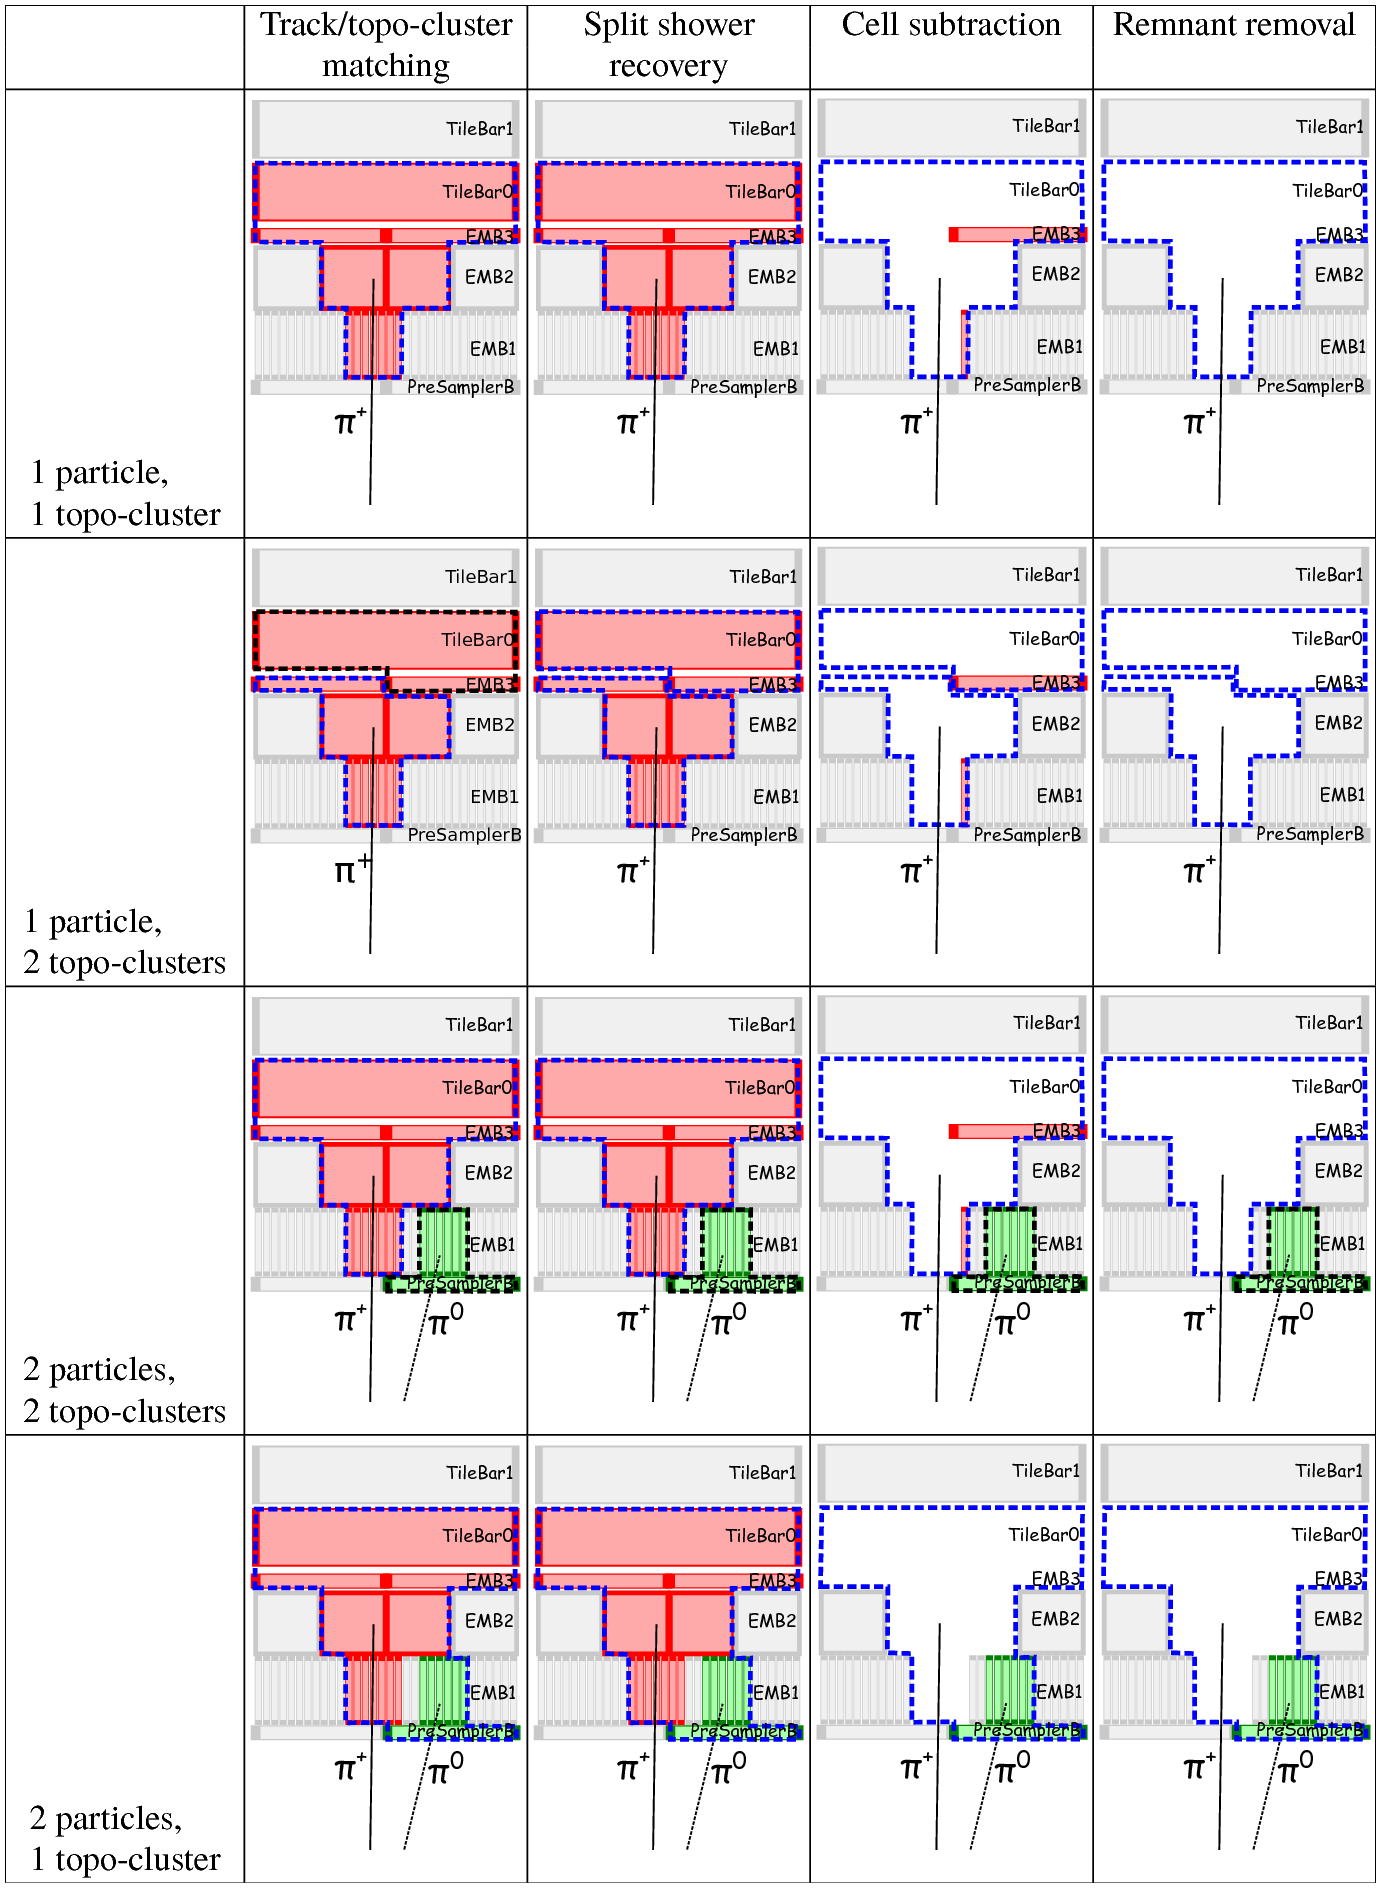
\includegraphics[width=0.8\textwidth]{figures/reco/reco_jets_pflow.png}
    \caption{Idealized example of how the PFlow algorithm is designed to deal with one or two pions creating one or two clusters in the ECal and TileCal. Red cells are those which have energy deposited from a $\pi^{+}$ and green cells are hits created from photons from the $\pi^{0}$ decay. Blue dotted lines represent clusters that have been matched by the algorithm to the $\pi^{+}$, while the black dotted lines have not been assigned. Taken from Ref.~\cite{ATLAS:2013eua}. }\label{fig:reco_pflow}
\end{figure}